\documentclass[spanish]{beamer}
\usepackage{graphicx}
\usepackage{multimedia}

% Tema de la presentación
\usetheme{metropolis}

% Información del documento
\title{Detección de defectos en objetos en movimiento mediante Redes Neuronales Convolucionales con optimizaciones específicas para hardware NVIDIA}

\date{11 de julio de 2025}
\author{Alumno: Haro Armero, Abel \\ Tutor: Flich Cardo, José \\ Co-tutor: López Rodríguez, Pedro Juan}

\titlegraphic{
\includegraphics[width=0.18\textwidth]{images/etsinf/logo-upv.pdf}\hfill
\includegraphics[width=0.18\textwidth]{images/etsinf/logo-etsinf.pdf}}

\setbeamertemplate{section in toc}[sections numbered]

\AtBeginSection{}


\begin{document}

% Diapositiva de título
\begin{frame}
    \titlepage
\end{frame}

\begin{frame}{Índice}
    \small\tableofcontents
\end{frame}

\section{Introducción}

\footnotesize
% En los últimos años, la Inteligencia Artificial ha crecido exponencialmente, impulsada por el aumento de datos, avances algorítmicos y mejoras en hardware como GPUs y TPUs. En especial, la visión por computador ha tenido un gran desarrollo gracias a las CNNs, con aplicaciones en seguridad, medicina o automoción. Sin embargo, este progreso plantea desafíos energéticos, lo que ha motivado la adopción de soluciones optimizadas como los dispositivos NVIDIA Jetson para tareas de IA eficientes en entornos embebidos. Este trabajo se centra en el desarrollo de un sistema de detección de defectos en objetos en movimiento utilizando CNNs, optimizado para hardware NVIDIA.
\begin{frame}{Introducción}
    \begin{columns}
        \begin{column}{0.45\textwidth}
            \begin{itemize}
                \item Crecimiento exponencial de la Inteligencia Artificial.
                \item Avances en visión por computador gracias a las CNNs.
                \item Desafíos energéticos impulsan soluciones optimizadas.
                \item Dispositivos NVIDIA Jetson para IA eficiente en entornos embebidos.
                \item Desarrollo de sistema de detección de defectos en objetos en movimiento con CNNs, optimizado para hardware NVIDIA.
            \end{itemize}
        \end{column}
        \begin{column}{0.5\textwidth}
            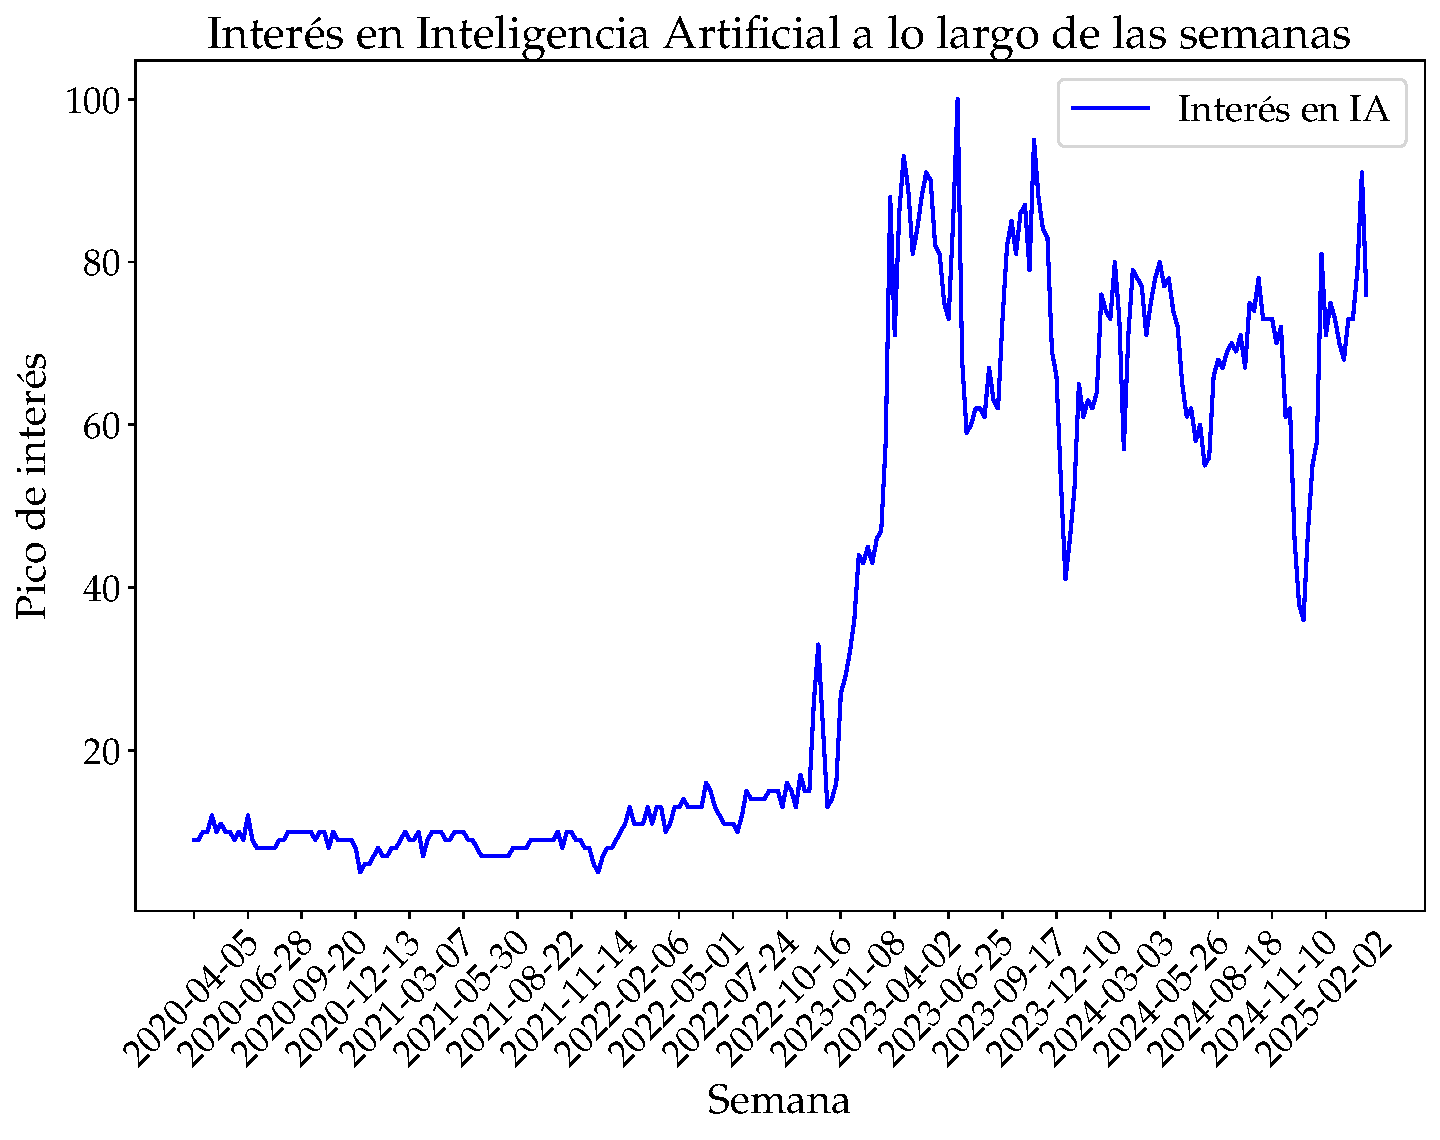
\includegraphics[width=0.95\textwidth]{images/introduccion/interes_en_ia.pdf}
            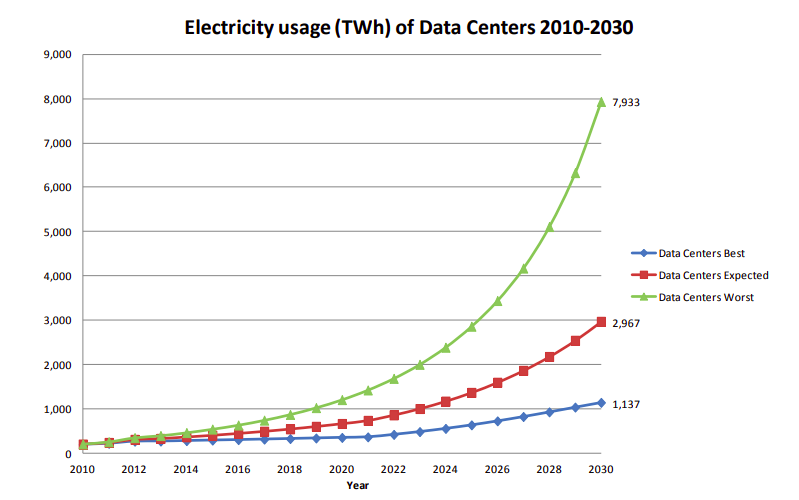
\includegraphics[width=0.95\textwidth]{images/introduccion/consumo_electrico_datacenters.png}
        \end{column}
    \end{columns}
\end{frame}


\section{Motivación}
% La visión por computador busca dotar a las máquinas de la capacidad de interpretar imágenes como lo hacen los humanos, siendo clave en la automatización industrial. Gracias a la IA y a dispositivos de bajo consumo como los Jetson de NVIDIA, es posible implementar soluciones eficientes en entornos de edge computing. Este trabajo se motiva en la necesidad de desarrollar un sistema que detecte y clasifique objetos en movimiento en cintas transportadoras, optimizando procesos y reduciendo errores.
\begin{frame}{Motivación}
    \begin{columns}
        \begin{column}{0.5\textwidth}
            \begin{itemize}
                \item Emular la interpretación humana de imágenes en máquinas.
                                    \item IA y visión por computador revolucionan la tecnología.
                                    \item NVIDIA Jetson impulsa la IA en edge computing.
                                    \item Automatización de la detección y clasificación de objetos en movimiento en la industria.
                            \end{itemize}
                        \end{column}

                        \begin{column}{0.5\textwidth}
                        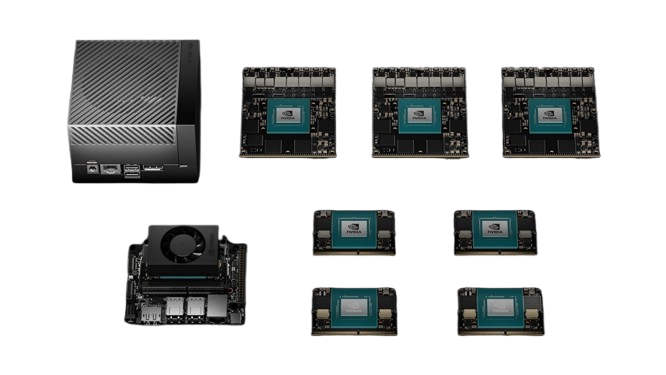
\includegraphics[width=0.95\textwidth]{images/motivacion/jetson_family.png}
                        \includegraphics[width=0.95\textwidth]{images/motivacion/quality_control.png}
                    \end{column}
                \end{columns}
            \end{frame}
            


% \section{Análisis del problema}
% \begin{frame}{Análisis del problema}
%     \begin{itemize}
%         \item Desarrollar un sistema de visión artificial para detectar defectos y realizar el seguimiento en tiempo real de múltiples objetos en movimiento.
%         \item Utilizar hardware NVIDIA Jetson por su eficiencia energética.
%         \item Emplear un entorno simulado con canicas de distintos colores y defectos para representar objetos en una línea de producción, ante la falta de un entorno industrial real.
%         \item Evaluar el rendimiento del sistema de forma controlada para su futura aplicación en escenarios industriales reales.
%         \end{itemize}
% \end{frame}

\section{Objetivos}
\begin{frame}{Objetivos}
    \begin{itemize}
        \item Estudiar el estado del arte en CNNs, aceleradores y optimización.
        \item Crear un conjunto de datos para entrenamiento y evaluación.
        \item Entrenar y validar modelos CNN para detección de defectos en tiempo real.
        \item Implementar un sistema de visión artificial integrado con hardware NVIDIA.
        \item Analizar y optimizar cuellos de botella para mejorar rendimiento y eficiencia.
        \item Evaluar el sistema con métricas de precisión, latencia y consumo.
        \item Realizar un análisis comparativo para encontrar la configuración óptima.
    \end{itemize}
\end{frame}

 \section{Conceptos previos}
            \begin{frame}{Conceptos Previos - Redes Neuronales Convolucionales (CNNs)}
                \begin{columns}
                    \begin{column}{0.5\textwidth}
                        \begin{itemize}
                            \item Las CNNs son un tipo de red neuronal profunda diseñadas para procesar datos con una estructura de cuadrícula, como imágenes.
                            \item El objetivo es localizar dentro de una imagen objetos y clasificarlos, detectando defectos o características específicas.
                            \item Utilizan capas convolucionales para extraer características jerárquicas.
                            \item Existen dos tipos principales de CNNs, detectores de dos etapas como R-CNN y detectores de una etapa como YOLO.
                            
                        \end{itemize}
                    \end{column}
        \begin{column}{0.5\textwidth}
            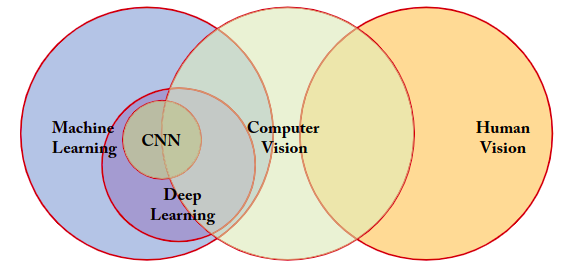
\includegraphics[width=0.95\textwidth]{images/conceptos_previos/diagrama_de_Venn_inteligencia_artificial.png}
            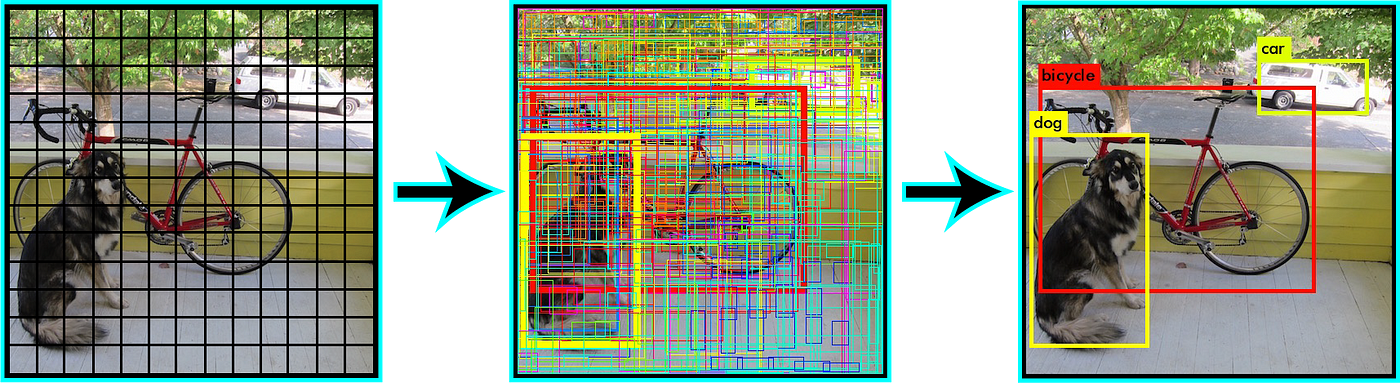
\includegraphics[width=0.95\textwidth]{images/conceptos_previos/yolo.png}
        \end{column}
    \end{columns}
\end{frame}


\begin{frame}{Conceptos Previos - Hardware NVIDIA Jetson}
    
    \begin{columns}
        \begin{column}{0.5\textwidth}
            \begin{itemize}
                \item Arquitecturas hardware especializadas para el deep learning.
                \item NVIDIA Jetson: SoC (System on a Chip) que integra CPU y GPU para eficiencia energética y procesamiento paralelo.
                %SDK Kit de desarrollo para crear aplicaciones de IA en dispositivos embebidos.
                \item Jetpack SDK y TensorRT: El SDK de NVIDIA proporiciona herramientas para desarrollar aplicaciones de IA, incluyendo TensorRT para optimizar de manera eficiente las redes neuronales en el hardware de NVIDIA.
            \end{itemize}
        \end{column}
        \begin{column}{0.5\textwidth}
            %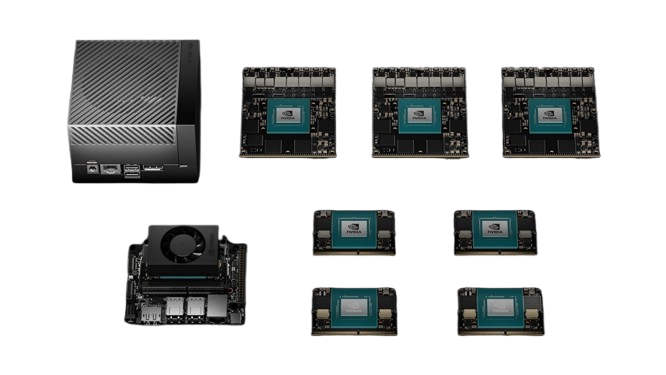
\includegraphics[width=0.95\textwidth]{images/motivacion/jetson_family.png}
            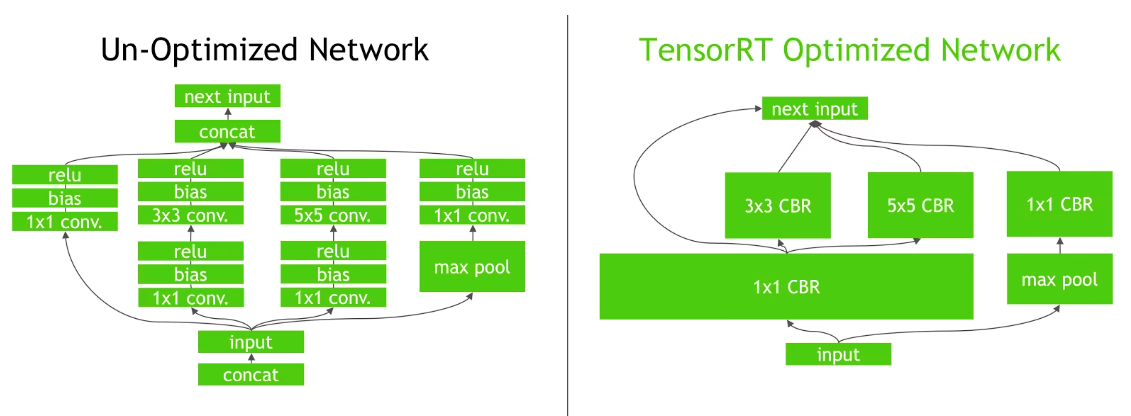
\includegraphics[width=1\textwidth]{images/conceptos_previos/TensorRT_optimizaciones.png}
            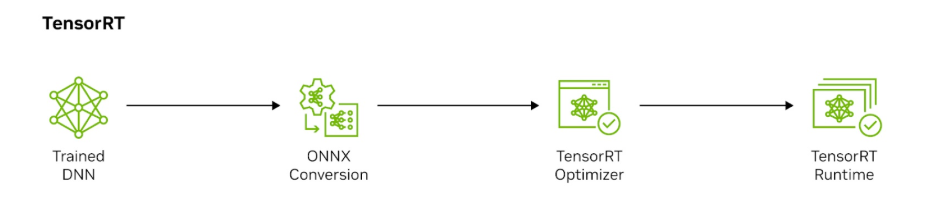
\includegraphics[width=1\textwidth]{images/conceptos_previos/TensorRT_pipeline.png}
        \end{column}
    \end{columns}
\end{frame}

\begin{frame}{Conceptos Previos - Seguimiento de objetos (MOT)}
    \begin{columns}
        \begin{column}{0.4\textwidth}
            \begin{itemize}
                \item El seguimiento de objetos es una técnica que permite identificar y seguir la trayectoria de un objeto a lo largo del tiempo en una secuencia de imágenes.
                \item Rastrea objetos combinando detección y análisis de movimiento.
                \item BYTETrack es el algoritmo de seguimiento que realiza el seguimiento de objetos a partir de las detecciones de un detector de objetos. 
            \end{itemize}
        \end{column}
        \begin{column}{0.7\textwidth}
            \includegraphics[width=1\textwidth]{images/conceptos_previos/tracking.png}
        \end{column}
    \end{columns}
   % \includegraphics[width=0.9\textwidth]{images/conceptos_previos/tracking.png}
\end{frame}


\section{Propuesta de solución}
\begin{frame}{Propuesta de solución}
    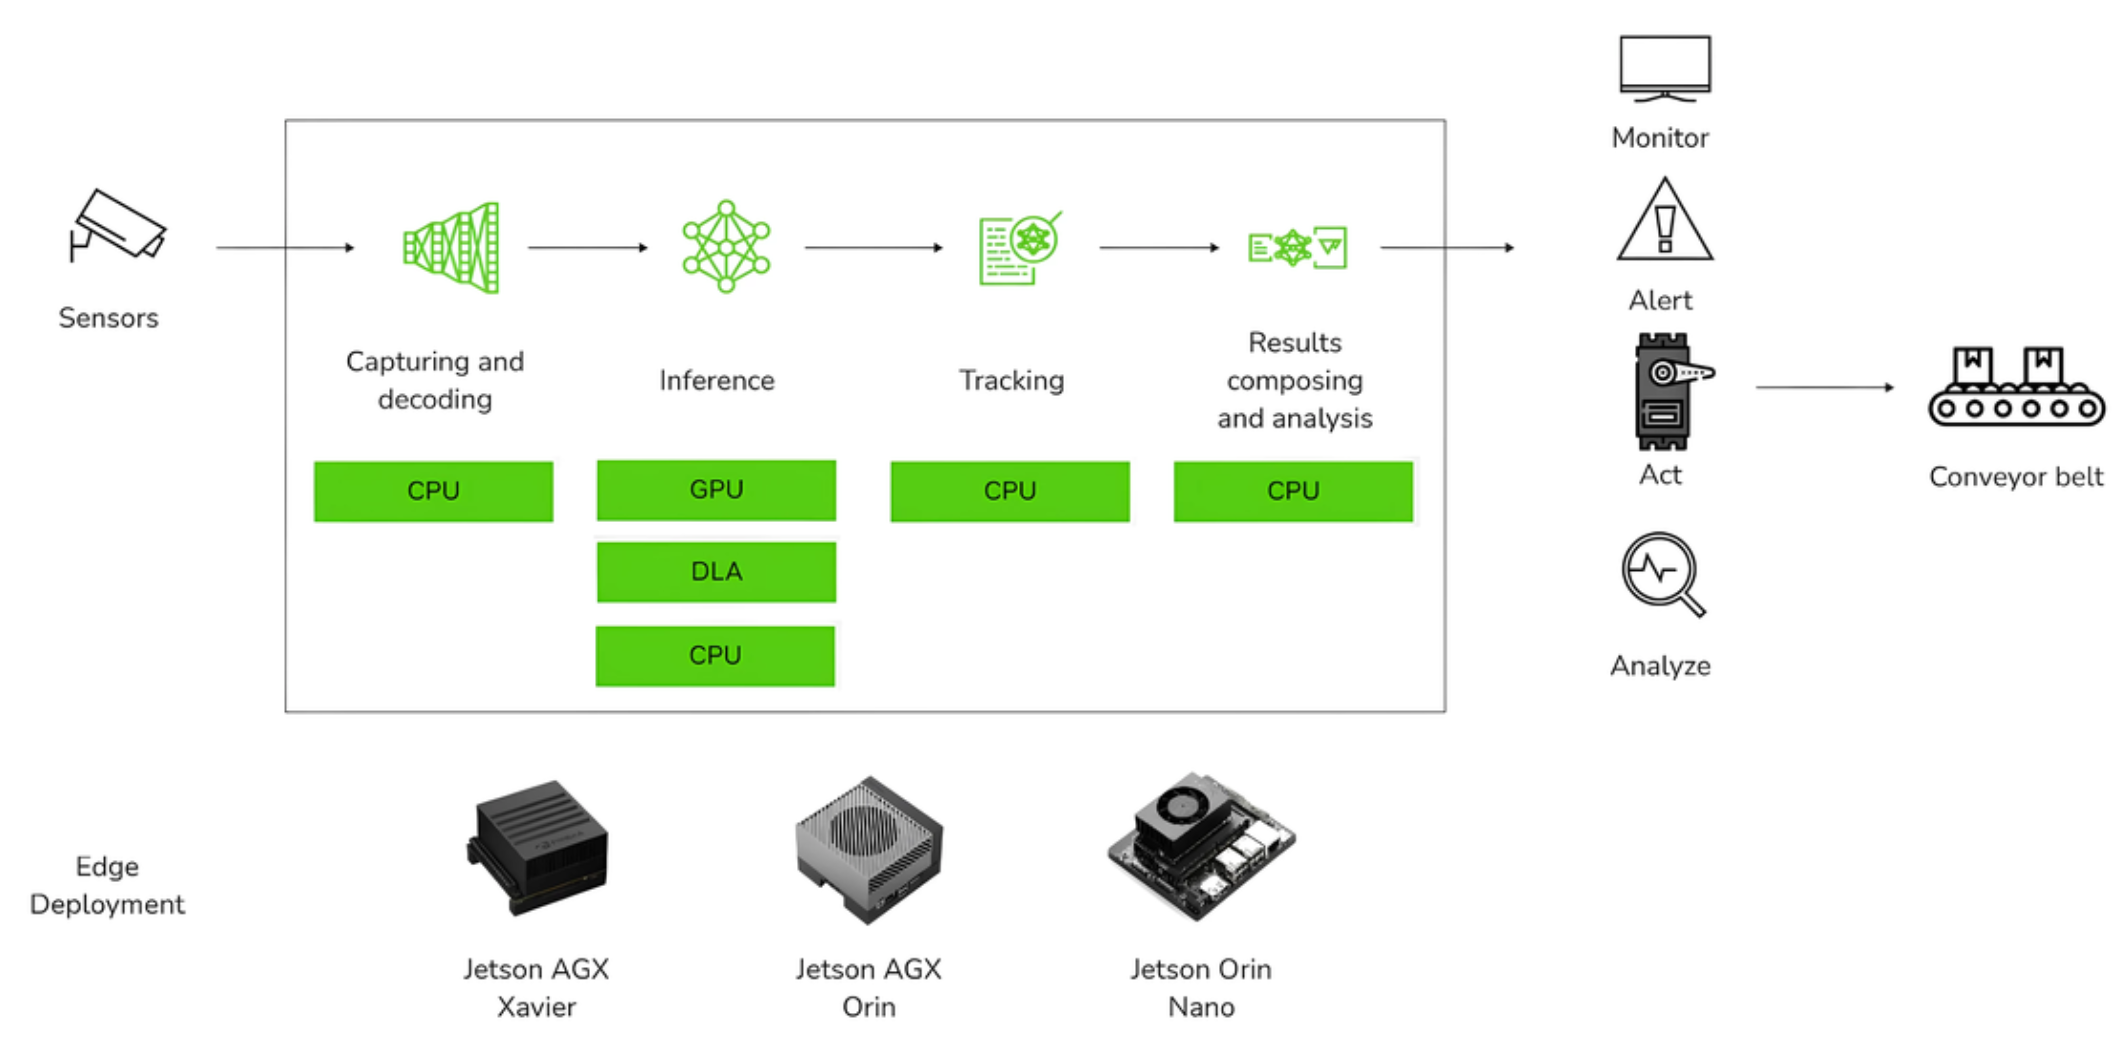
\includegraphics[width=0.9\textwidth]{images/solucion_propuesta/figura_TFG_v3.png}
\end{frame}

\section{Desarrollo de la solución}

\begin{frame}{Desarrollo de la solución - Entrenamiento y validación de modelos}
    \begin{columns}
        \begin{column}{0.5\textwidth}
            \begin{itemize}
                \item Creación de un conjunto de datos con imágenes de canicas de distintos colores y defectos.
                \item Entrenamiento de modelos CNN para detección de defectos.
                \item Validación y ajuste de hiperparámetros para mejorar precisión.
                \item Exportación de los modelos a TensorRT para optimizar su rendimiento en hardware NVIDIA.
            \end{itemize}
        \end{column}
        \begin{column}{0.5\textwidth}
            \begin{center}
                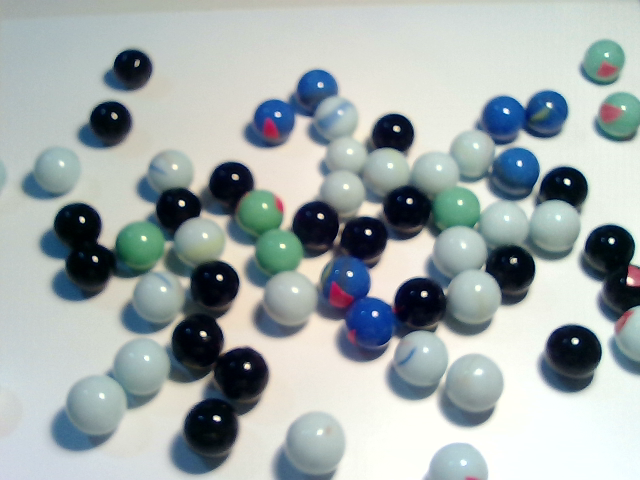
\includegraphics[width=0.8\textwidth]{images/solucion_propuesta/ejemplo_canicas.png}
                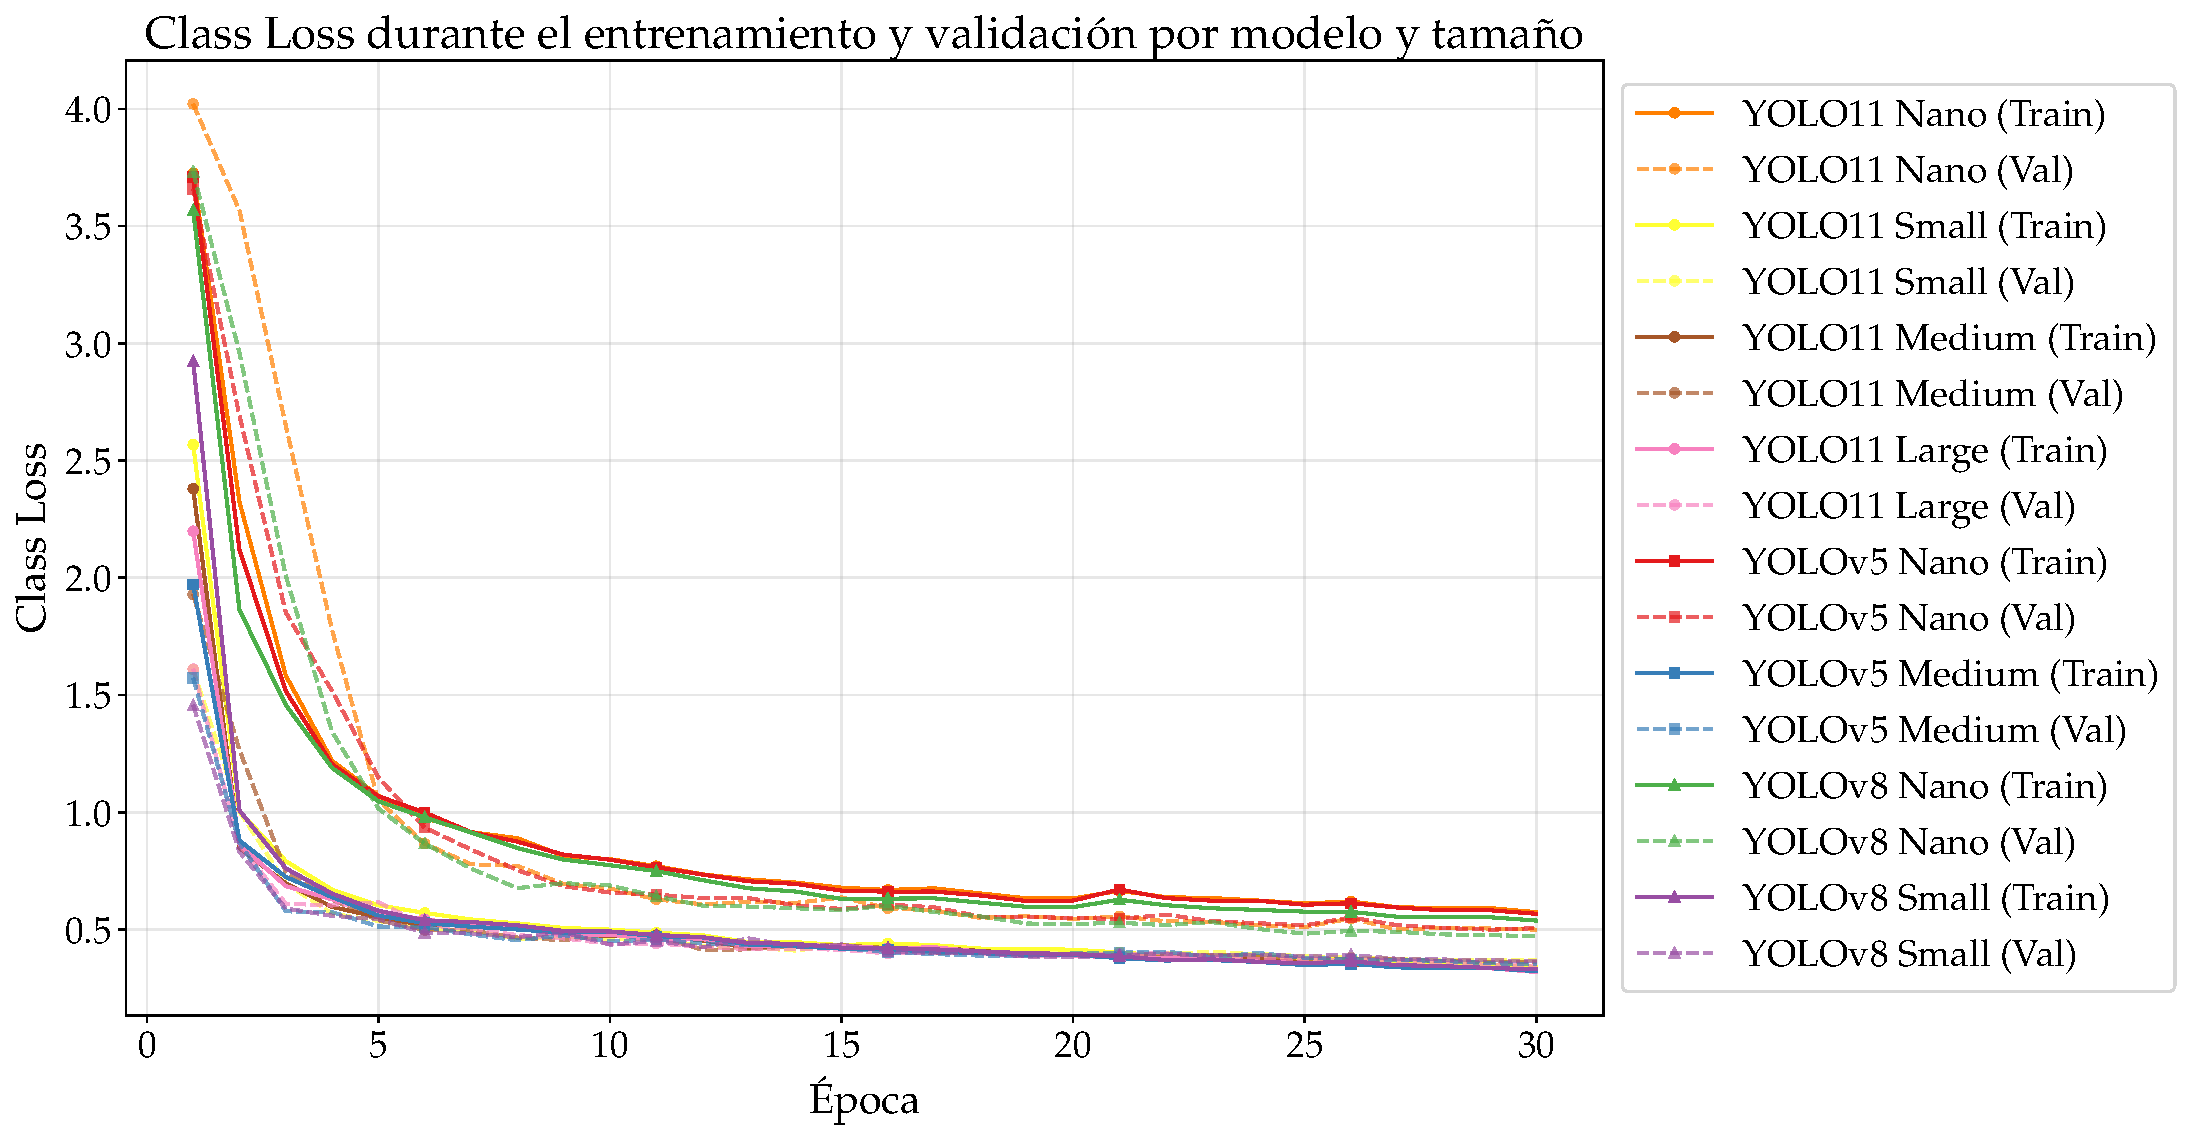
\includegraphics[width=0.95\textwidth]{images/solucion_propuesta/loss_plot.pdf}
            \end{center}
        \end{column}
    \end{columns}
\end{frame}

\begin{frame}{Desarrollo de la solución - Segmentación de las etapas (1/5)}
    \begin{itemize}
        \item El sistema se divide en cuatro etapas, captura de vídeo, detección de objetos, seguimiento de objetos y visualización.
        \item El objetivo de segmentar las etapas es permitir que cada una de ellas operen de forma independiente para mejorar la velocidad y eficiencia del sistema.
        \item Se han propuesto cuatro formas de segmentación para mejorar el procesamiento secuencial, (1) segmentación por \textbf{hilos}, (2) segmentación por \textbf{procesos}, (3) segmentación por \textbf{procesos con memoria compartida} y (4) segmentación por \textbf{heterogénea}
    \end{itemize}
    \begin{center}
        \begin{center}
            
            \begin{figure}
                \centering
                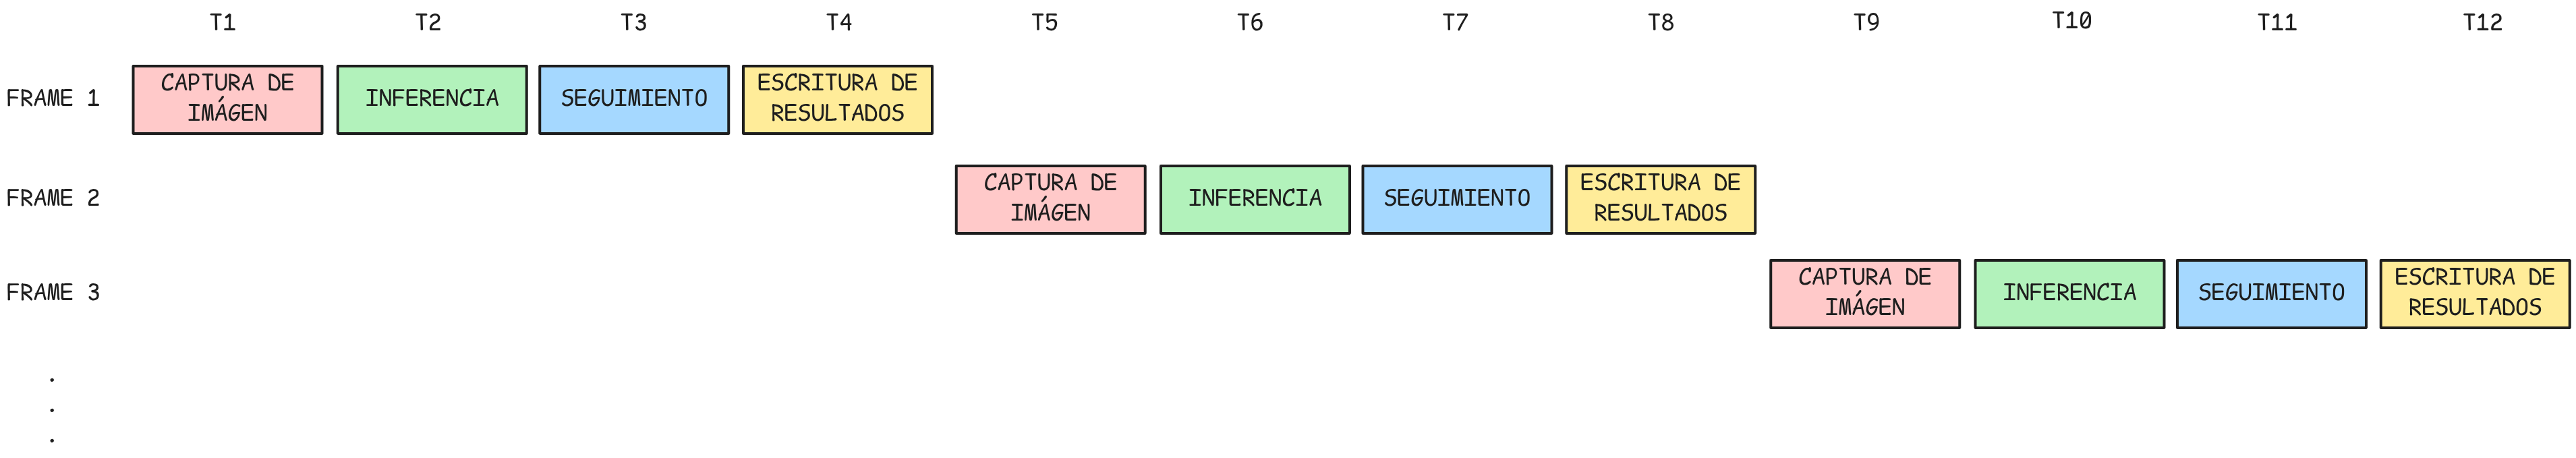
\includegraphics[width=0.9\textwidth]{images/solucion_propuesta/secuencial.png}
                \vspace{0.5cm}
                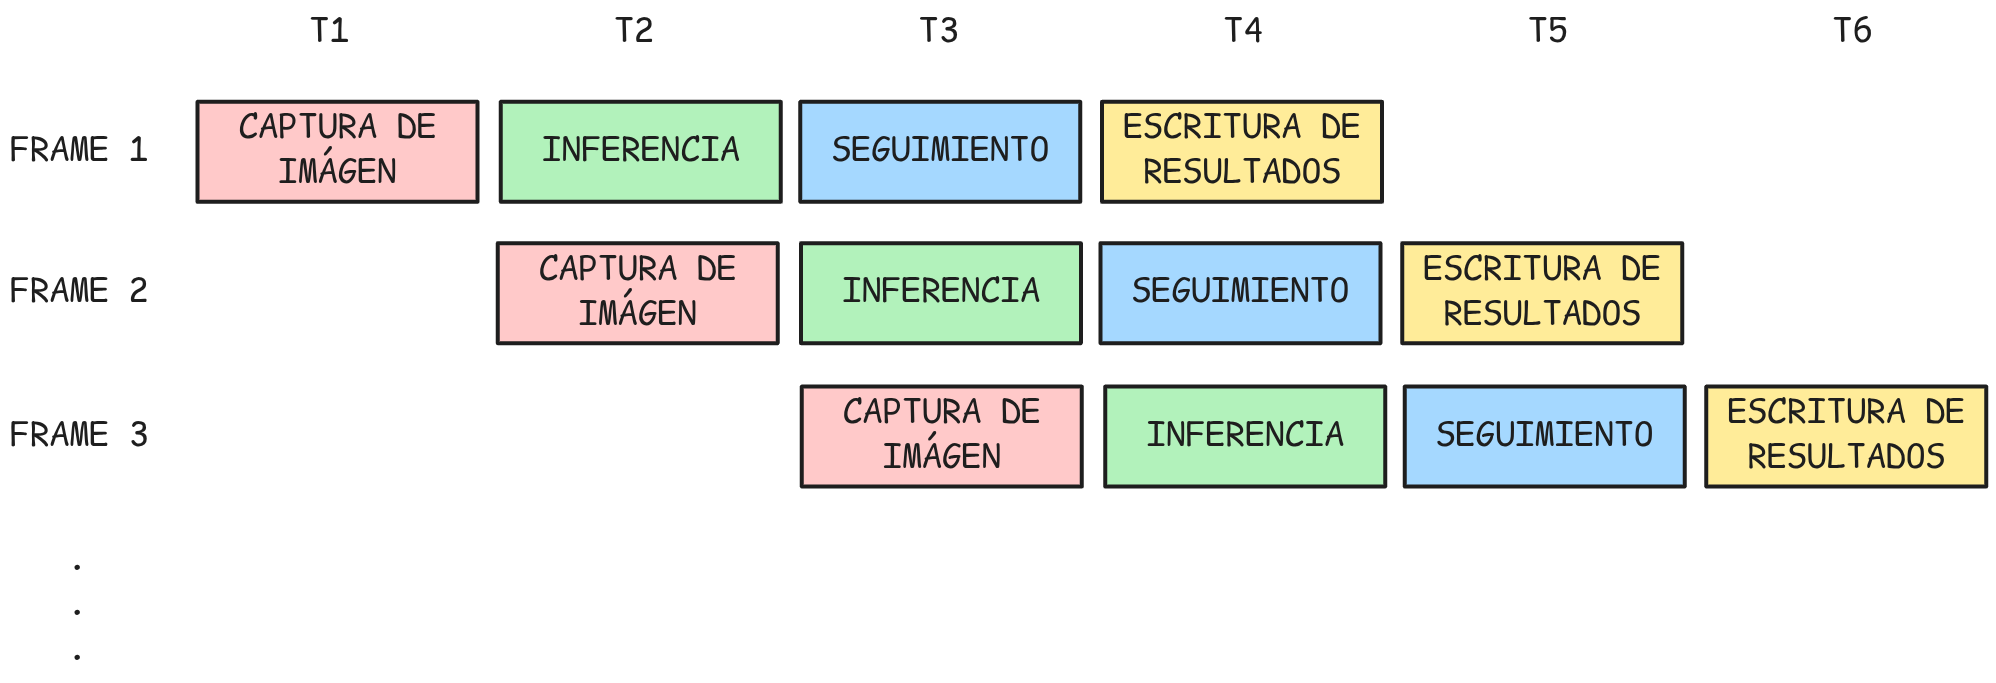
\includegraphics[width=0.55\textwidth]{images/solucion_propuesta/segmentacion.png}
            \end{figure}
        \end{center}
    \end{center}
\end{frame}

\begin{frame}{Desarrollo de la solución - Segmentación de las etapas (2/5)}
    \begin{columns}
        \begin{column}{0.5\textwidth}
            \textbf{Segmentación por hilos:}
            \begin{itemize}
                \item Cada etapa se ejecuta en un hilo separado.
                \item La información se comparte entre hilos mediante colas que se consumen de forma asíncrona.
                \item Permite un procesamiento paralelo pero no concurrente debido al GIL (Global Interpreter Lock) de Python.
            \end{itemize}
        \end{column}
        \begin{column}{0.5\textwidth}
            \begin{center}
                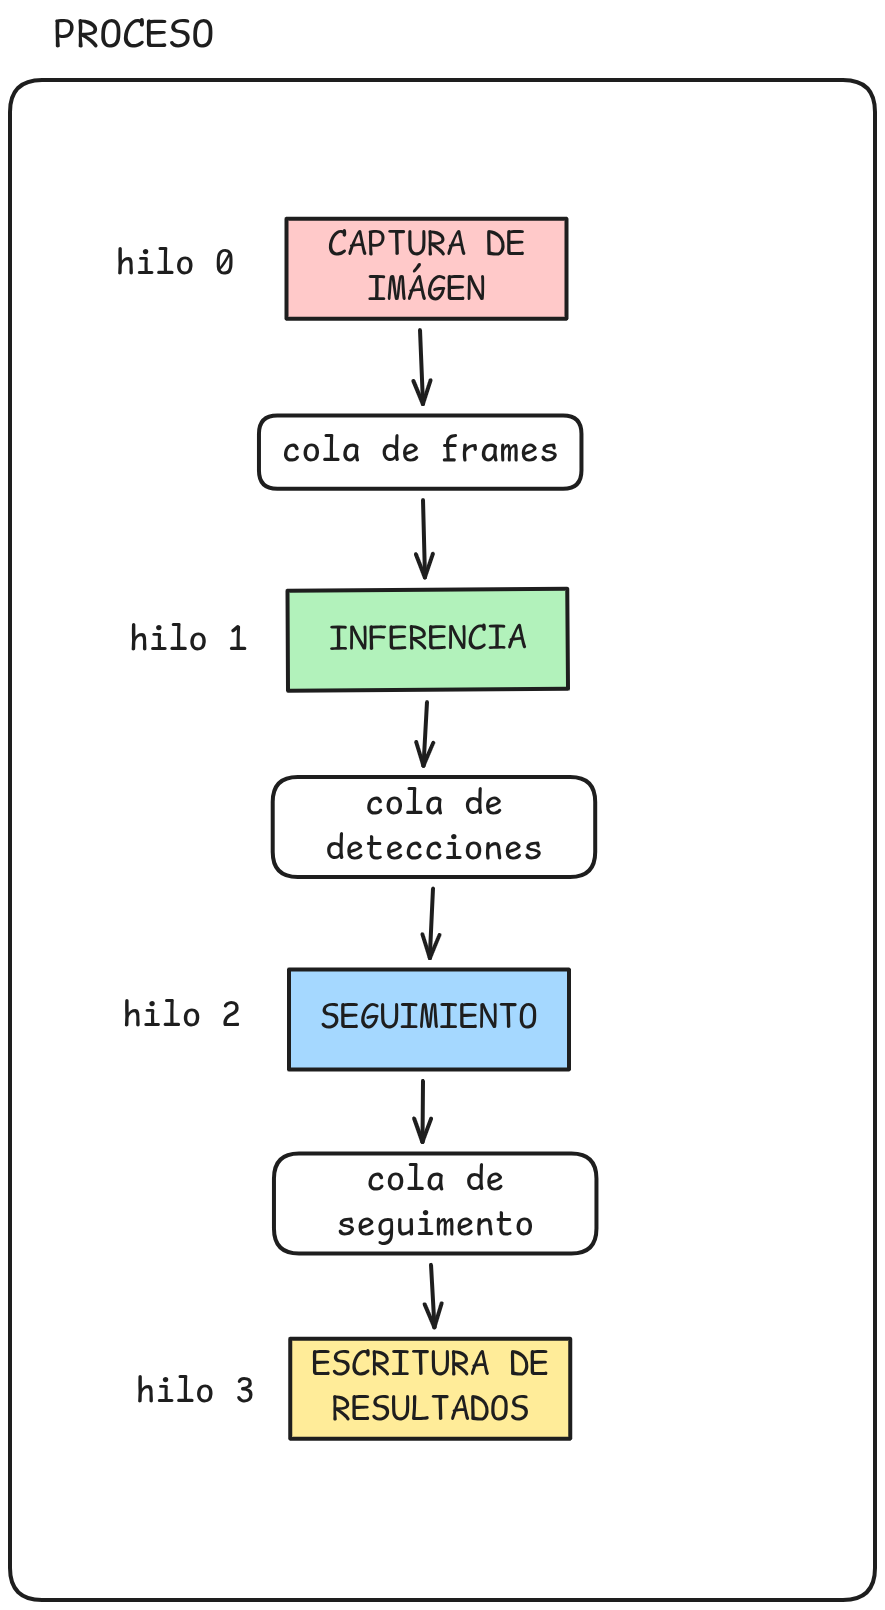
\includegraphics[width=0.75\textwidth]{images/solucion_propuesta/segmentacion_hilos.png}
            \end{center}
        \end{column}
    \end{columns}

\end{frame}

\begin{frame}{Desarrollo de la solución - Segmentación de las etapas (3/5)}
    \begin{columns}
        \begin{column}{0.5\textwidth}
            \textbf{Segmentación por procesos:}
            \begin{itemize}
                \item Cada etapa se ejecuta en un proceso separado.
                \item La comunicación entre procesos se realiza mediante colas implementadas sobre pipes.
                \item Permite un procesamiento concurrente, pero con mayor latencia en la comunicación.
        \end{itemize}
        \end{column}
            \begin{column}{0.5\textwidth}
            \begin{center}
                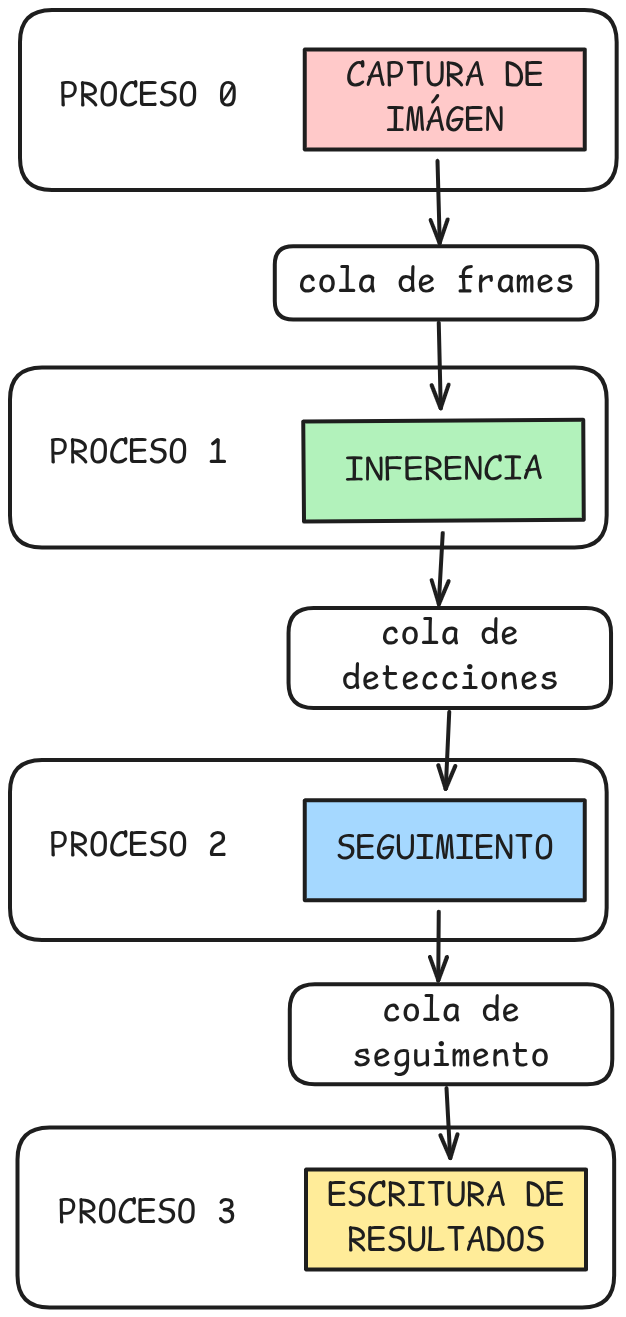
\includegraphics[width=0.7\textwidth]{images/solucion_propuesta/segmentacion_procesos.png}
            \end{center}
        \end{column}
    \end{columns}

\end{frame}

\begin{frame}{Desarrollo de la solución - Segmentación de las etapas (4/5)}
    \begin{columns}
        \begin{column}{0.5\textwidth}
            \textbf{Segmentación por procesos con memoria compartida:}
            \begin{itemize}
                \item Cada etapa se ejecuta en un proceso separado, pero comparten memoria.
                \item Las colas de comunicación se implementan sobre memoria entre procesos evitando la sobrecarga de pipes.
                \item Permite un procesamiento concurrente con menor latencia en la comunicación.
            \end{itemize}
        \end{column}
        \begin{column}{0.5\textwidth}
                \begin{center}
                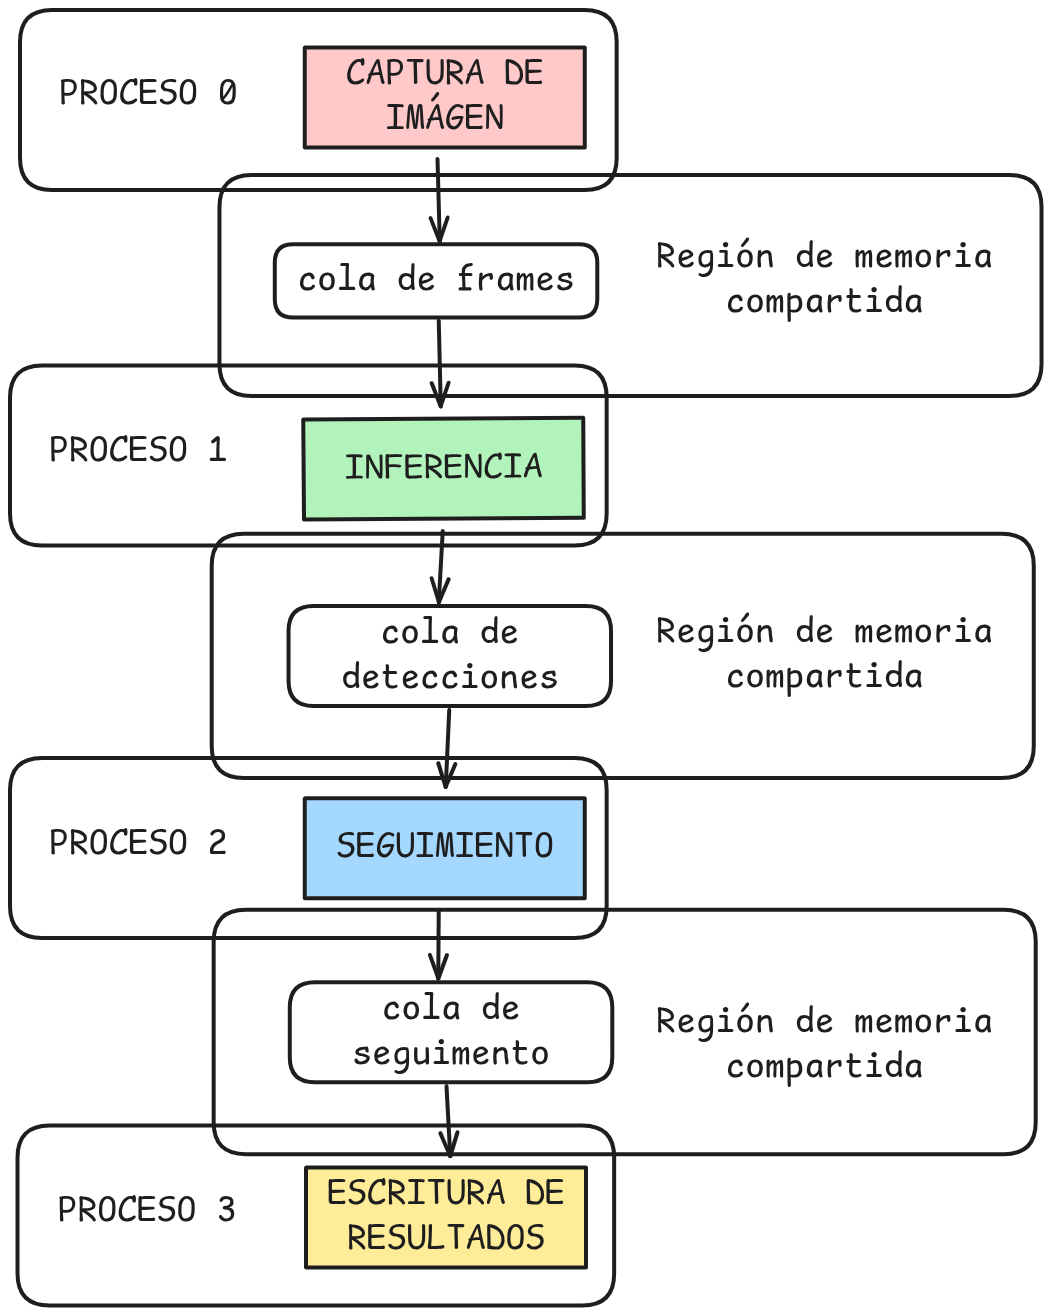
\includegraphics[width=0.8\textwidth]{images/solucion_propuesta/segmentacion_procesos_memoria_compartida.png}
            \end{center}
        \end{column}
    \end{columns}
\end{frame}

\begin{frame}{Desarrollo de la solución - Segmentación de las etapas (5/5)}
    \begin{columns}
        \begin{column}{0.5\textwidth}
            \textbf{Segmentación por heterogénea:}
            \begin{itemize}
                \item Se puede ejecutar tanto con hilos como con procesos (con y sin memoria compartida).
                \item Ejecuta la etapa de de detección en la GPU o DLAs del dispositivo Jetson.
                \item Permite explotar todos los recursos para mejorar el rendimiento.
                \item Los modelos de no se ejecutan completamente en la DLA.
            \end{itemize}
        \end{column}
        \begin{column}{0.5\textwidth}
            \begin{center}
                %\includegraphics[width=0.8\textwidth]{images/solucion_propuesta/segmentacion_heterogenea.png}
                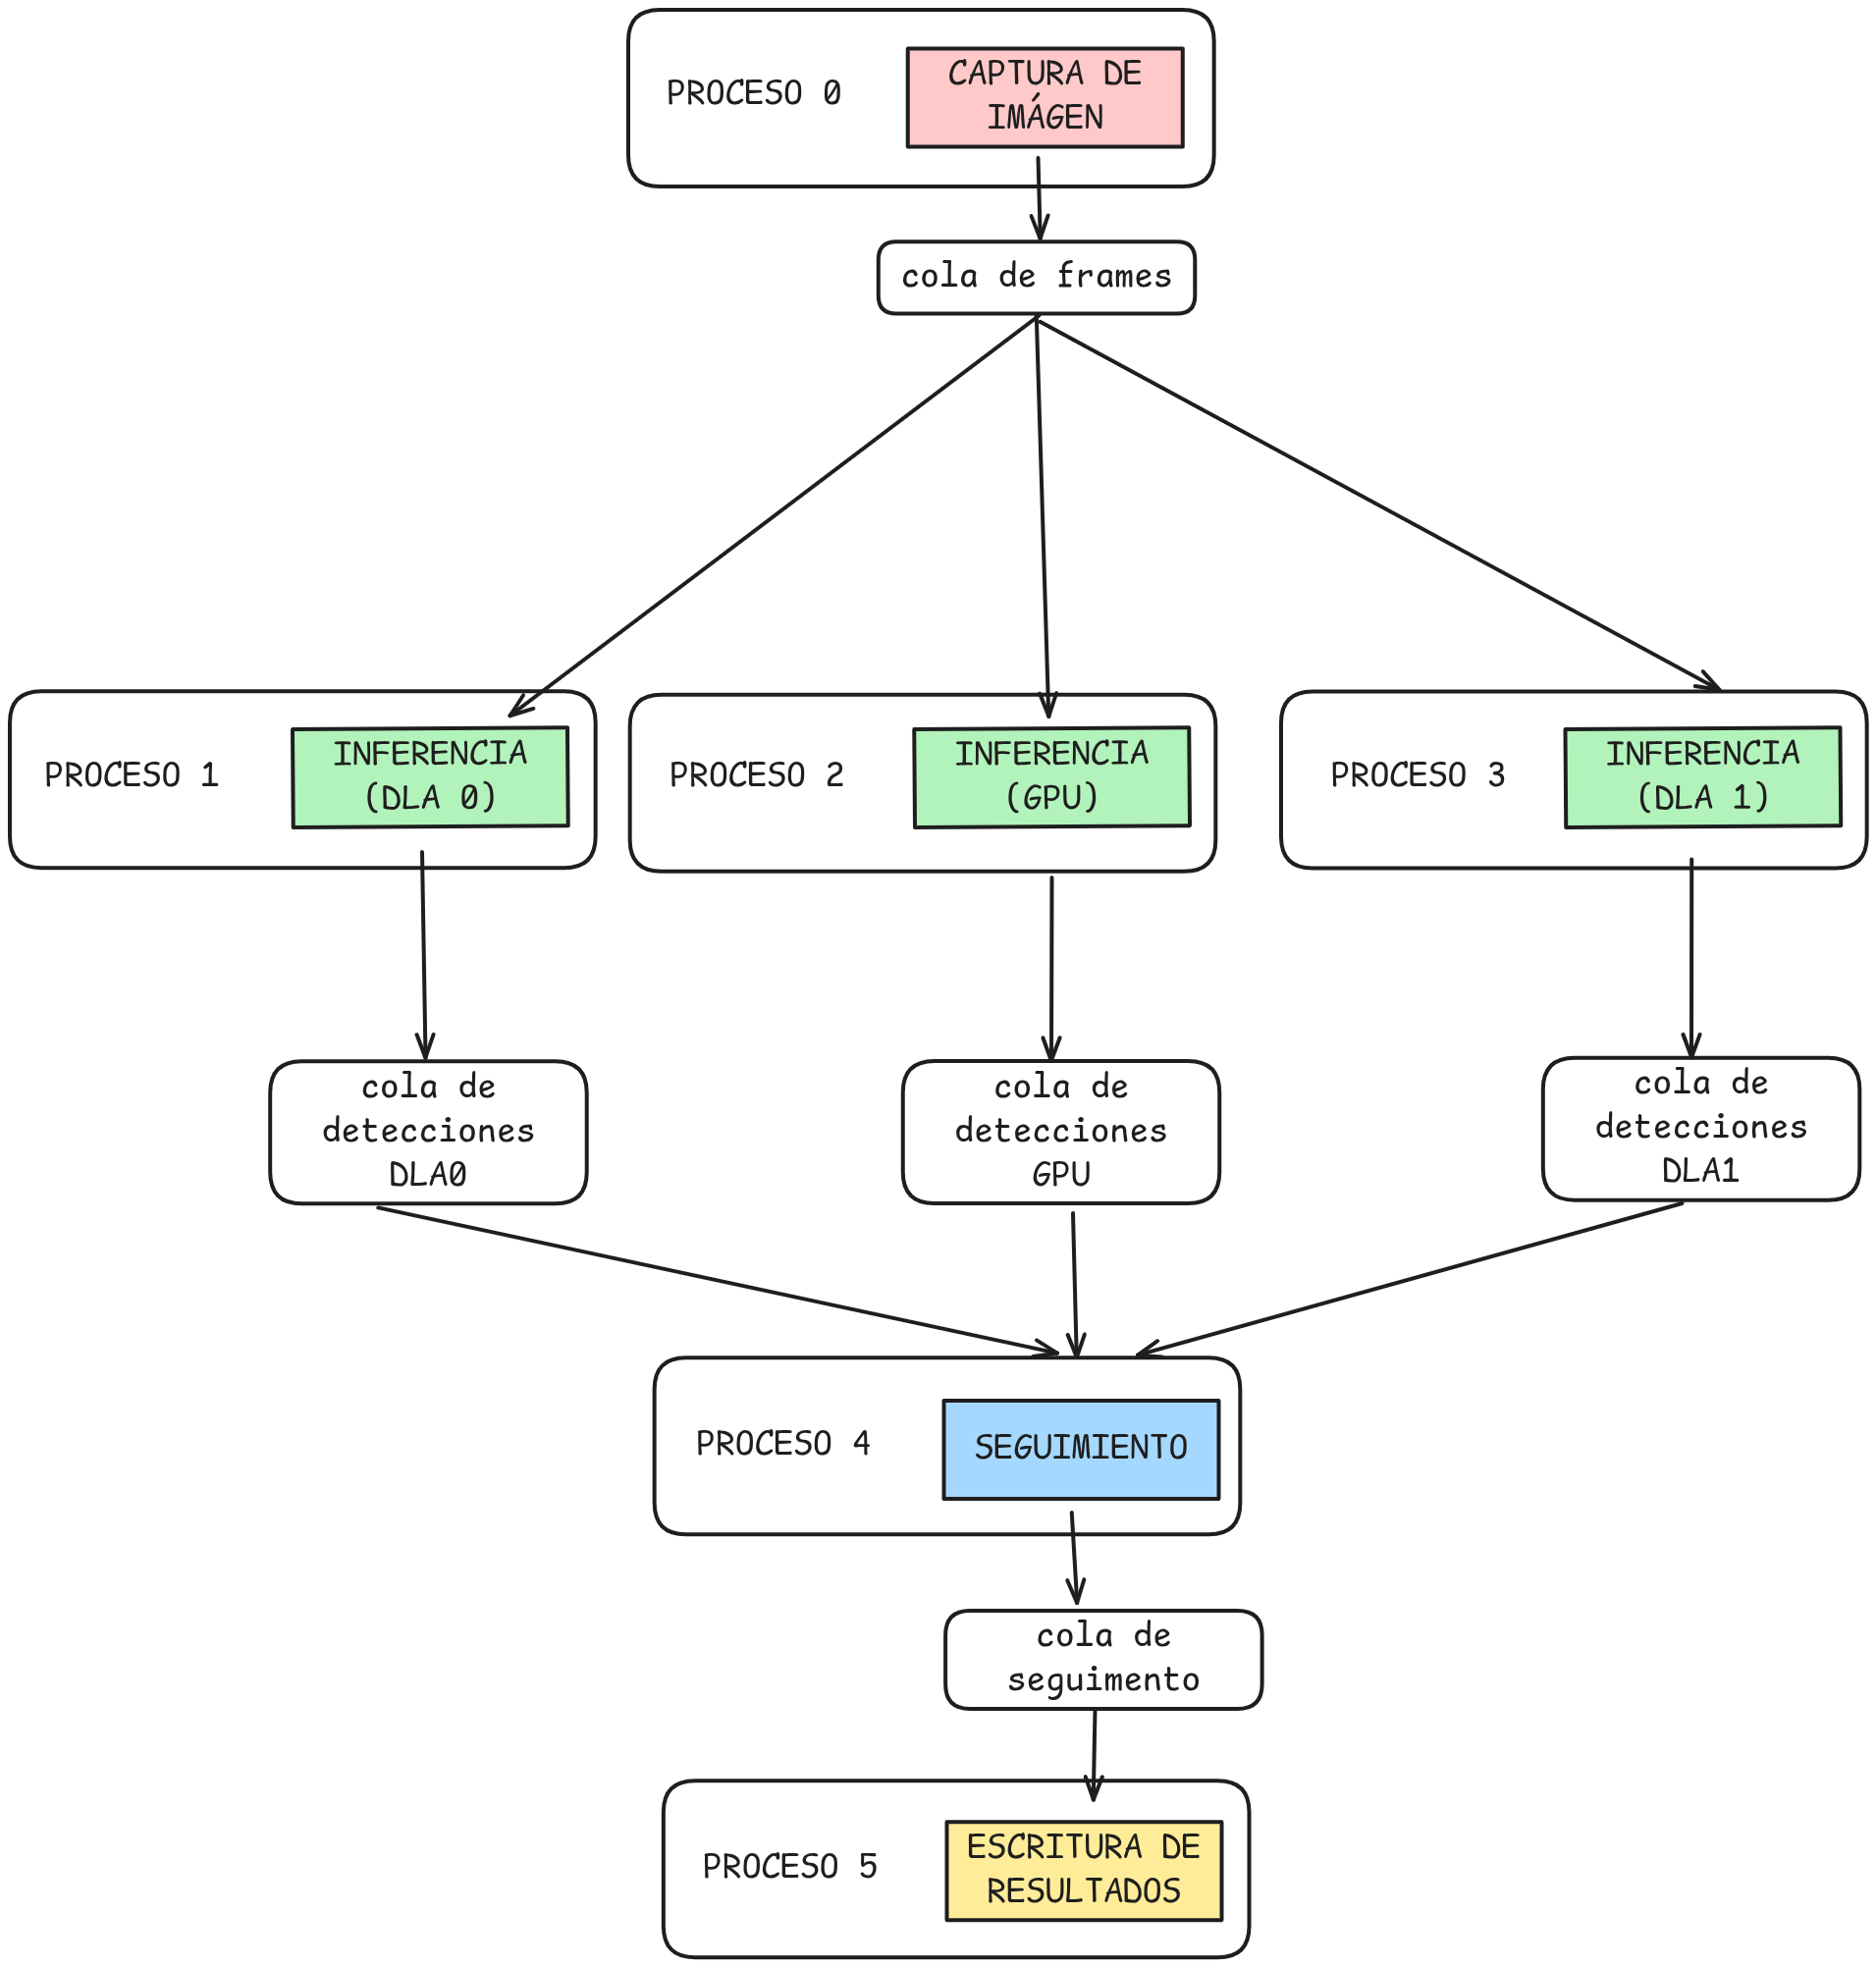
\includegraphics[width=0.8\textwidth]{images/solucion_propuesta/segmentacion_multihardware.png}
            \end{center}
        \end{column}
    \end{columns}
\end{frame}

\begin{frame}{Desarrollo de la solución - Prueba de concepto}
    \begin{columns}
        \begin{column}{0.5\textwidth}
            Como prueba simple de concepto, se ha construido una pequeña cinta transportadora con un motor. El sistema captura el vídeo de la cinta transportadora y detecta canicas de distintos colores y defectos. El objetivo es demostrar que el sistema es capaz de detectar objetos en movimiento y clasificarlos en tiempo real.


        \end{column}
        \begin{column}{0.5\textwidth}
            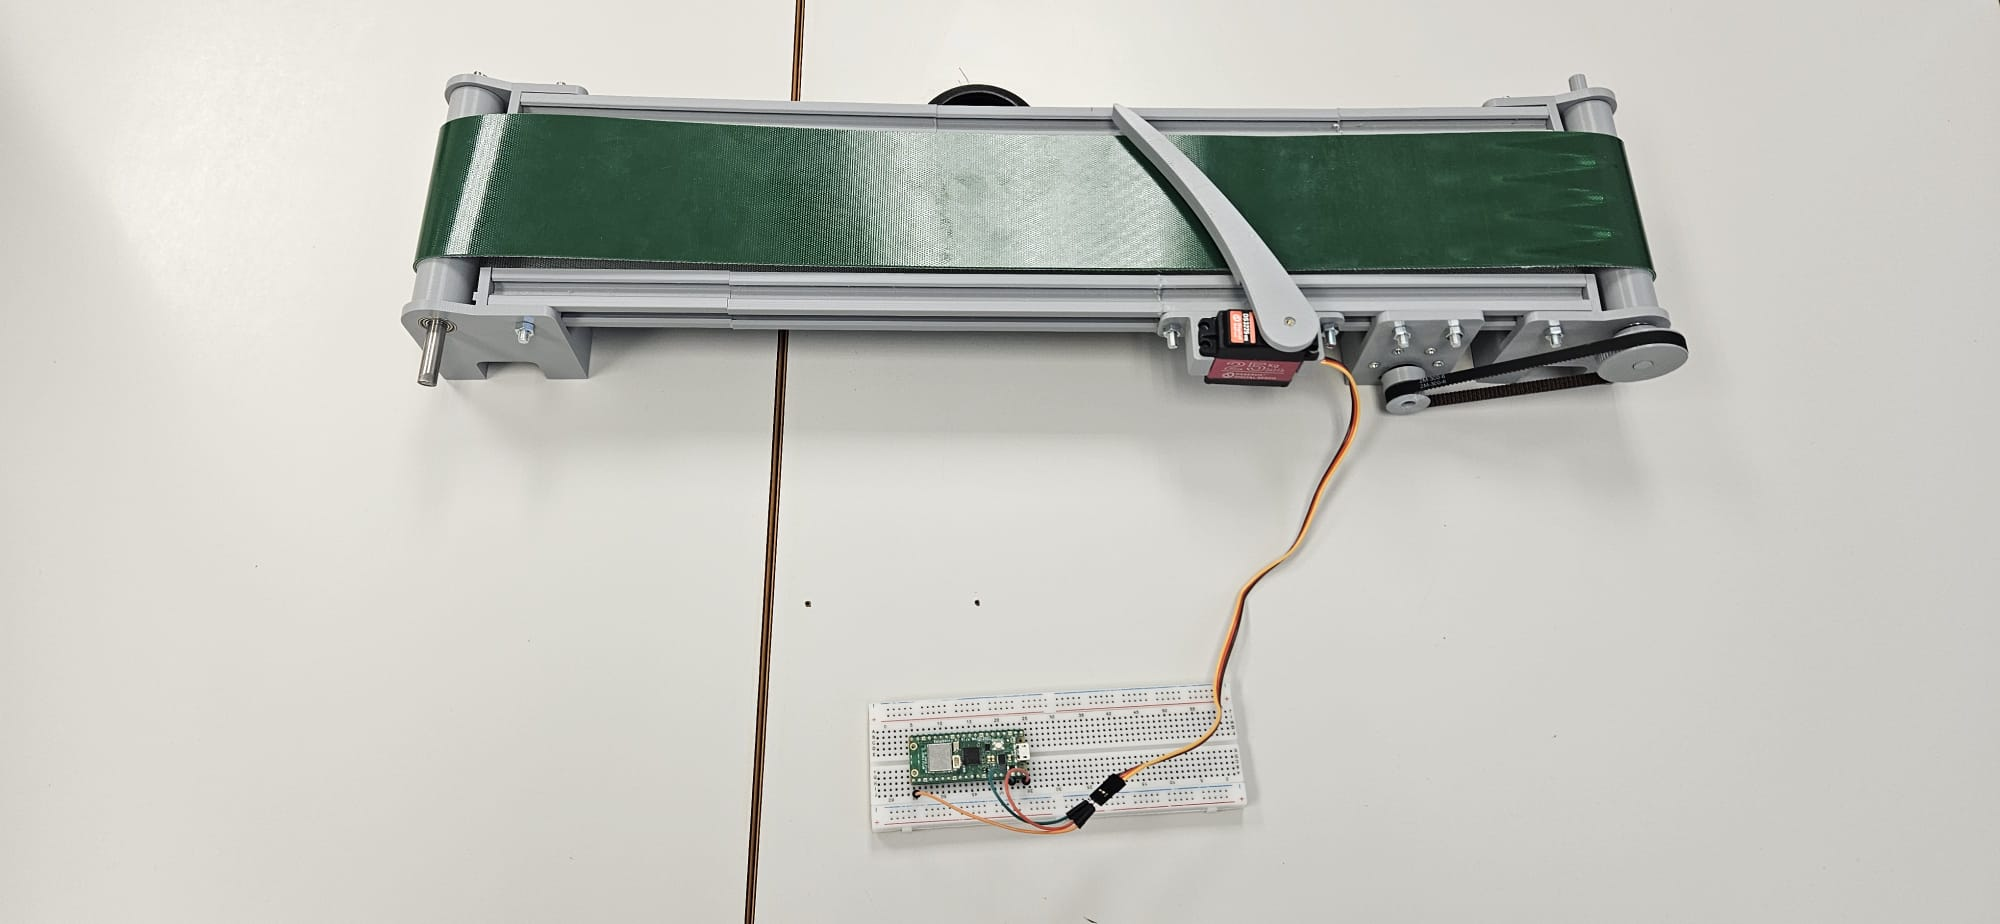
\includegraphics[width=0.95\textwidth]{images/solucion_propuesta/cinta_transportadora_construccion.jpeg}
        \end{column}
    \end{columns}
\end{frame}

\section{Demo del sistema}
\begin{frame}{Demo del sistema}
    \begin{center}
        % Video con texto como placeholder
        \movie[width=0.8\textwidth,height=0.6\textwidth,showcontrols]{
            \fbox{\parbox{0.8\textwidth}{\centering\vspace{2cm}
            \Huge \textbf{VIDEO DEMO}\\[0.5cm]
            \Large Sistema de detección de defectos\\[0.3cm]
            \normalsize Haz clic para reproducir
            \vspace{2cm}}}}
        {demo/demo_defensa.mp4}
    \end{center}
\end{frame}


\section{Resultados}
\begin{frame}{Resultados}
    \begin{itemize}
        \item Para evaluar el rendimiento del sistema, se han realizado pruebas con diferentes configuraciones de segmentación y optimización. Los resultados se han medido en términos de precisión, latencia y consumo energético.
        \item Existen todas estas configuraciones para evaluar el rendimiento del sistema:
        \begin{itemize}
            \item Cantidad de objetos media en el vídeo.
            \item Tipo de segmentación: hilos, procesos, procesos con memoria compartida y heterogénea.
            \item Tipo de modelo y talla: YOLOv5{nu, mu}, YOLOv8{n, s} y YOLO11{n, s, m, l}.
            \item Precisión del modelo: FP32, FP16 y INT8.
            \item Modo de energía del dispositivo Jetson (MAXN, 30W8core, 30W4core, 15W4core, etc). 
            \item Dispositivo Jetson: Jetson AGX Xavier, Jetson AGX Orin y Jetson Orin Nano.
    \end{itemize}
    \end{itemize}
\end{frame}

\begin{frame}{Resultados - Cantidad de objetos}
    \begin{columns}
        \begin{column}{0.5\textwidth}
            \begin{itemize}
                \item Se ha evaluado el rendimiento del sistema con diferentes cantidades de objetos en el vídeo.
                \item 4 vídeos, (1) media de 17 objetos, (2) media de 43 objetos, (3) media de 84 objetos y (4) carga variable de 0 a 180 objetos.
                \item Para el resto de la configuración se ha utilizado los parámetros más óptimos encontrados en la sección de análisis comparativo.
            \end{itemize}
        \end{column}
        \begin{column}{0.5\textwidth}
        \end{column}
    \end{columns}
\end{frame}


\begin{frame}{Resultados - Tipo de segmentación}
    \begin{columns}
        \begin{column}{0.5\textwidth}
            \begin{itemize}
                \item Se ha evaluado el rendimiento del sistema con diferentes tipos de segmentación.
                \item Se han utilizado los vídeos con una media de 17 objetos y 43 objetos.
                \item Para el resto de la configuración se ha utilizado los parámetros más óptimos encontrados en la sección de análisis comparativo.
            \end{itemize}
        \end{column}
        \begin{column}{0.5\textwidth}

        \end{column}
    \end{columns}
\end{frame}

\section{Conclusiones}
\begin{frame}{Conclusiones -- Cumplimiento de objetivos (1/3)}
    \textbf{Los objetivos del TFG se han alcanzado con éxito:}
    \begin{itemize}
        \item \textbf{Estudio del estado del arte:} Se realizó un análisis exhaustivo de CNNs, aceleradores hardware y plataformas NVIDIA Jetson, superando desafíos de compatibilidad y configuración en arquitectura ARM64.
        \item \textbf{Creación del conjunto de datos:} Se generó un dataset y vídeos de entrenamiento que simulan condiciones reales de operación con objetos de variabilidad controlada.
        \item \textbf{Entrenamiento de modelos CNN:} Se entrenaron múltiples modelos de las familias YOLOv5, YOLOv8 y YOLO11 en diversas precisiones, optimizando hiperparámetros mediante iteraciones exhaustivas.
    \end{itemize}
\end{frame}

\begin{frame}{Conclusiones -- Cumplimiento de objetivos (2/3)}
    \begin{itemize}
        \item \textbf{Implementación del sistema integrado:} Se desarrolló un sistema de visión artificial que combina detección con seguimiento BYTETrack, manteniendo la identidad de objetos a lo largo del tiempo.
        \item \textbf{Análisis y optimización de cuellos de botella:} Se exploraron estrategias de segmentación (hilos, procesos, memoria compartida, heterogénea), identificando la segmentación por procesos con memoria compartida como la más efectiva.
        \item \textbf{Evaluación con métricas completas:} Se realizaron experimentos exhaustivos evaluando precisión, latencia y consumo en diferentes configuraciones de hardware Jetson.
    \end{itemize}
\end{frame}

\begin{frame}{Conclusiones -- Logros y desafíos superados (3/3)}
    \textbf{Principales logros alcanzados:}
    \begin{itemize}
        \item Sistema funcional de detección de defectos en tiempo real optimizado para hardware NVIDIA\@.
        \item Configuración estable del entorno de desarrollo superando incompatibilidades de frameworks.
        \item Integración exitosa de detección y seguimiento con mejoras significativas en precisión y robustez.
        \item Identificación de configuraciones óptimas mediante análisis comparativo exhaustivo.
    \end{itemize}
    
    \vspace{0.5cm}
    
    \textbf{Desafíos técnicos superados:}
    \begin{itemize}
        \item Gestión de compatibilidad entre versiones de frameworks de deep learning.
        \item Programación concurrente y gestión de memoria compartida interproceso.
        \item Optimización de rendimiento mediante ajuste fino de hiperparámetros.
    \end{itemize}
\end{frame}

\begin{frame}
    \titlepage
\end{frame}

\end{document}








% % Primera sección
% \section{A}

% \begin{frame}{¿Qué es LaTeX Beamer?}
%     \begin{itemize}
%         \item Beamer es una clase de LaTeX para crear presentaciones
%         \item Permite crear diapositivas profesionales
%         \item Muy utilizado en el ámbito académico
%         \item Soporte completo para matemáticas: $E = mc^2$
%     \end{itemize}
% \end{frame}

% % Segunda sección
% \section{Características principales}

% \begin{frame}{Ventajas de Beamer}
%     \begin{enumerate}
%         \item \textbf{Control total} sobre el formato
%         \item \textbf{Consistencia} en el diseño
%         \item \textbf{Ecuaciones} matemáticas perfectas
%         \item \textbf{Referencias} automáticas
%     \end{enumerate}
    
%     \vspace{1cm}
    
%     \begin{block}{Ejemplo de bloque}
%         Los bloques son útiles para destacar información importante.
%     \end{block}
% \end{frame}

% \begin{frame}{Ejemplo con columnas}
%     \begin{columns}
%         \begin{column}{0.5\textwidth}
%             \textbf{Columna izquierda:}
%             \begin{itemize}
%                 \item Punto 1
%                 \item Punto 2
%                 \item Punto 3
%             \end{itemize}
%         \end{column}
        
%         \begin{column}{0.5\textwidth}
%             \textbf{Columna derecha:}
%             \begin{itemize}
%                 \item Otro punto 1
%                 \item Otro punto 2
%                 \item Otro punto 3
%             \end{itemize}
%         \end{column}
%     \end{columns}
% \end{frame}

% % Tercera sección
% \section{Conclusiones}

% \begin{frame}{Conclusiones}
%     \begin{alertblock}{Importante}
%         Beamer es una excelente herramienta para presentaciones académicas.
%     \end{alertblock}
    
%     \vspace{0.5cm}
    
%     \begin{itemize}
%         \item Fácil de aprender
%         \item Resultados profesionales
%         \item Altamente personalizable
%     \end{itemize}
    
%     \vspace{1cm}
    
%     \centering
%     \Large ¡Gracias por su atención!
% \end{frame}

% \end{document}